% Created 2018-04-30 seg 11:34
% Intended LaTeX compiler: pdflatex
\documentclass[presentation]{beamer}
\usepackage[utf8]{inputenc}
\usepackage[T1]{fontenc}
\usepackage{graphicx}
\usepackage{grffile}
\usepackage{longtable}
\usepackage{wrapfig}
\usepackage{rotating}
\usepackage[normalem]{ulem}
\usepackage{amsmath}
\usepackage{textcomp}
\usepackage{amssymb}
\usepackage{capt-of}
\usepackage{hyperref}
\usepackage{graphicx, hyperref, udesc, url}
\usetheme{default}
\author{Rafael Castro}
\date{03/05/2018}
\title{Aula 1 de Coq}
\hypersetup{
 pdfauthor={Rafael Castro},
 pdftitle={Aula 1 de Coq},
 pdfkeywords={},
 pdfsubject={},
 pdfcreator={Emacs 25.3.1 (Org mode 9.1.11)}, 
 pdflang={Portuguese}}
\begin{document}

\maketitle

\section{Introducao}
\label{sec:org02d2f72}

\begin{frame}[label={sec:orgb3ccb78}]{Provadores Automáticos}
\begin{itemize}
\item Entre com uma proposição, aperte um botão e veja a resposta.
\item Fazem todo o trabalho da prova. Humanos não são necessários.
\item Limitados a domínios específicos.
\item São procedimentos de decisão.
\item Fornecem um formalismo para especificar a proposição, mas não para a sua prova. Fornecem uma valoração caso falso.
\end{itemize}
\end{frame}
\begin{frame}[label={sec:org0d7e165}]{Assistentes de Provas}
\begin{itemize}
\item São provadores semi-automáticos.
\item Uso com domínio menos restrito: podem falar sobre diversas lógicas, teorias e até mesmo programas.
\item Podem utilizar provadores automáticos, mas ainda necessitam do humano.
\item Fornecem um formalismo para representar a prova. \emph{Lembra} as regras da Dedução.
\end{itemize}
\end{frame}

\begin{frame}[label={sec:orge460205}]{Como Assistentes de provas assistem?}
\begin{itemize}
\item O núcleo de um assistente de provas é um verificador, que verifica a consistência lógica da prova.
\item Fornecem de maneira interativa de visualizar as informações sobre o estado atual da prova.
\item Ajudam a encontrar teoremas e lemas para o progresso da prova.
\item Permitem implementar métodos não-deterministas para auxiliar a prova.
\end{itemize}
\end{frame}

\begin{frame}[label={sec:orgea5ae09}]{Qual assistente utilizar?}
\begin{itemize}
\item Existem diversos assistentes, cada um baseado numa teoria matemática e com as suas peculiaridades:
Agda, Isabelle, HOL, Minlog, Coq\ldots{}
\item Iremos utilizar Coq! Mas por que?
\begin{enumerate}
\item É o que eu sei algo;
\item Existe desde 1984;
\item Há vários livros.
\item Suporte para ordem superior, tipos dependentes, automação e extração de código.
\end{enumerate}
\end{itemize}
\end{frame}

\begin{frame}[label={sec:org8cbc353}]{Como aprender Coq?}
Vamos utilizar o Volume 1 do Software Foundations 
\url{https://softwarefoundations.cis.upenn.edu/}
\begin{center}
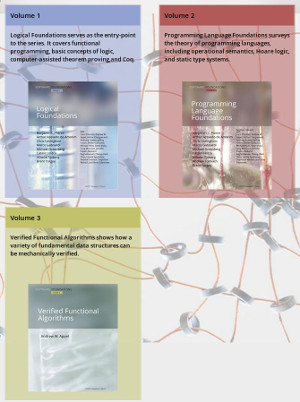
\includegraphics[width=.9\linewidth]{./sf.jpeg}
\end{center}
\end{frame}

\section{Baby's First Steps}
\label{sec:org88a10b5}

\begin{frame}[label={sec:org2b95eba}]{Como utilizar o assistente de provas?}
\begin{itemize}
\item CoqIDE = Bom lugar para começar sem perder o foco. Tem os recursos básicos.
\item Emacs + ProofGeneral + Company-coq =
\end{itemize}
\end{frame}
\end{document}